%%%%%%%%%%%%%%%%%%%%%%%%%%%%%%%%%%%%%%%%%
% BEng Internship Report
% Representation and writing of my internship report in LaTeX
% Version 1.0 01st Jan, 2016
%%%%%%%%%%%%%%%%%%%%%%%%%%%%%%%%%%%%%%%%%

%----------------------------------------------------------------------------------------
%	PACKAGES AND OTHER DOCUMENT CONFIGURATIONS
%----------------------------------------------------------------------------------------

\documentclass[
11pt, % The default document font size, options: 10pt, 11pt, 12pt
%oneside, % Two side (alternating margins) for binding by default, uncomment to switch to one side
english, % ngerman for German
singlespacing, % Single line spacing, alternatives: onehalfspacing or doublespacing
%draft, % Uncomment to enable draft mode (no pictures, no links, overfull hboxes indicated)
%nolistspacing, % If the document is onehalfspacing or doublespacing, uncomment this to set spacing in lists to single
%liststotoc, % Uncomment to add the list of figures/tables/etc to the table of contents
%toctotoc, % Uncomment to add the main table of contents to the table of contents
%parskip, % Uncomment to add space between paragraphs
%nohyperref, % Uncomment to not load the hyperref package
headsepline, % Uncomment to get a line under the header
]{InternshipReport} % The class file specifying the document structure

\usepackage[utf8]{inputenc} % Required for inputting international characters
\usepackage[T1]{fontenc} % Output font encoding for international characters

\usepackage{palatino} % Use the Palatino font by default

\usepackage[backend=bibtex,style=authoryear,natbib=true]{biblatex} % User the bibtex backend with the authoryear citation style (which resembles APA)

\addbibresource{example.bib} % The filename of the bibliography

\usepackage[autostyle=true]{csquotes} % Required to generate language-dependent quotes in the bibliography

%----------------------------------------------------------------------------------------
%	MARGIN SETTINGS
%----------------------------------------------------------------------------------------

\geometry{
	paper=a4paper, % Change to letterpaper for US letter
	inner=2.5cm, % Inner margin
	outer=3.8cm, % Outer margin
	bindingoffset=2cm, % Binding offset
	top=1.5cm, % Top margin
	bottom=1.5cm, % Bottom margin
	%showframe,% show how the type block is set on the page
}

%----------------------------------------------------------------------------------------
%	THESIS INFORMATION
%----------------------------------------------------------------------------------------

\thesistitle{Module Development of a SaaS platform (Nukeboard)} % Your thesis title, this is used in the title and abstract, print it elsewhere with \ttitle
\supervisor{Dr. Nde \textsc{Nguti}} % Your supervisor's name, this is used in the title page, print it elsewhere with \supname
\examiner{} % Your examiner's name, this is not currently used anywhere in the template, print it elsewhere with \examname
\degree{Bachelor of Engineering } % Your degree name, this is used in the title page and abstract, print it elsewhere with \degreename
\author{Alangi \textsc{Derick}} % Your name, this is used in the title page and abstract, print it elsewhere with \authorname
\addresses{} % Your address, this is not currently used anywhere in the template, print it elsewhere with \addressname

\subject{Software Engineering} % Your subject area, this is not currently used anywhere in the template, print it elsewhere with \subjectname
\keywords{} % Keywords for your thesis, this is not currently used anywhere in the template, print it elsewhere with \keywordnames
\university{\href{http://www.ubuea.net}{University Of Buea, Bachelor of Engineering Program}} % Your university's name and URL, this is used in the title page and abstract, print it elsewhere with \univname
\department{\href{http://www.ubuea.net}{Department of Computer Engineering}} % Your department's name and URL, this is used in the title page and abstract, print it elsewhere with \deptname
\faculty{Faculty of Engineering and Technology} % Your faculty's name and URL, this is used in the title page and abstract, print it elsewhere with \facname

\hypersetup{pdftitle=\ttitle} % Set the PDF's title to your title
\hypersetup{pdfauthor=\authorname} % Set the PDF's author to your name
\hypersetup{pdfkeywords=\keywordnames} % Set the PDF's keywords to your keywords

\begin{document}

\frontmatter % Use roman page numbering style (i, ii, iii, iv...) for the pre-content pages

\pagestyle{plain} % Default to the plain heading style until the thesis style is called for the body content

%----------------------------------------------------------------------------------------
%	TITLE PAGE
%----------------------------------------------------------------------------------------

\begin{titlepage}
\begin{center}

\textsc{\LARGE \univname}\\[1.5cm] % University name
\textsc{\Large Internship Report}\\[0.5cm] % Thesis type

\HRule \\[0.4cm] % Horizontal line
{\huge \bfseries \ttitle}\\[0.4cm] % Thesis title
\HRule \\[1cm] % Horizontal line

\textsc{\Large offered by \LARGE Njorku, Cameroon}\\[1.2cm] % Thesis type
 

\begin{minipage}{0.4\textwidth}
\begin{flushleft} \large
\emph{Author:}\\
{\authorname, (FE12A113), \\ alangiderick@gmail.com} % Author name - remove the \href bracket to remove the link
\end{flushleft}
\end{minipage}
\begin{minipage}{0.4\textwidth}
\begin{flushright} \large
\emph{Supervisor:} \\
{Dr Nde Nguti} % Supervisor name - remove the \href bracket to remove the link  
\end{flushright}
\end{minipage}\\[1.8cm]

\textsc{\Large performed at \LARGE Njorku, Cameroon}\\[2.0cm] % Thesis type
 
\large \textit{A report submitted in partial fulfillment of the requirements of \\ \degreename degree programme in Computer Engineering} \\[1.2cm] % University requirement text

\large{Report of Internship from 1st September, 2015 to 31st January, 2016}\\[2cm]
 
{\large \today}\\[4cm] % Date
%\includegraphics{Logo} % University/department logo - uncomment to place it
 
\vfill
\end{center}
\end{titlepage}

%----------------------------------------------------------------------------------------
%	DECLARATION PAGE
%----------------------------------------------------------------------------------------

\begin{declaration}
\addchaptertocentry{\authorshipname}

\noindent I, \authorname, declare that this report titled, \enquote{\ttitle} and the work presented in it are my own. I confirm that:

\begin{itemize} 
\item This work was done wholly or mainly while in candidature for a bachelors degree at this University.
\item Where any part of this report has previously been submitted for a degree or any other qualification at this University or any other institution, this has been clearly stated.
\item Where I have consulted the published work of others, this is always clearly attributed.
\item Where I have quoted from the work of others, the source is always given. With the exception of such quotations, this thesis is entirely my own work.
\item I have acknowledged all main sources of help.
\item Where the report is based on work done by myself jointly with others, I have made clear exactly what was done by others and what I have contributed myself.\\
\end{itemize}
 
\noindent Signed:\\
\rule[0.5em]{25em}{0.5pt} % This prints a line for the signature
 
\noindent Date:\\
\rule[0.5em]{25em}{0.5pt} % This prints a line to write the date
\end{declaration}

\cleardoublepage

%----------------------------------------------------------------------------------------
%	QUOTATION PAGE
%----------------------------------------------------------------------------------------

\vspace*{0.2\textheight}

\noindent\enquote{\itshape Thanks to my solid academic training, today I can write hundreds of words on virtually any topic without possessing a shared of information, which is how I got a good training and reputation in the my domain of studies and in the industrial world in and out of the country.}\bigbreak

\hfill \authorname

%----------------------------------------------------------------------------------------
%	ABSTRACT PAGE
%----------------------------------------------------------------------------------------

\begin{abstract}
\addchaptertocentry{\abstractname} % Add the abstract to the table of contents

The Report Abstract is written here (and usually kept to just this page). The page is kept centered vertically so can expand into the blank space above the title too\ldots

\end{abstract}

%----------------------------------------------------------------------------------------
%	ACKNOWLEDGEMENTS
%----------------------------------------------------------------------------------------

\begin{acknowledgements}
\addchaptertocentry{\acknowledgementname} % Add the acknowledgements to the table of contents

I would like to express my deepest appreciation to all those who provided me the possibility to complete this report. A special gratitude I give to internship project manager, Mr. William Mukete, whose contributions in stimulating suggestions and encouragement, helped me to coordinate my project especially in writing this report.

Furthermore I would also like to acknowledge with much appreciation the crucial role of the staff of {\facname}, who gave the permission to use all required equipment and the necessary materials to complete the  task \enquote{\ttitle}. A special thanks goes to my team mate, Fonji Fonkeng Rocard, with whom i worked in collaboration with on the project “Nukeboard”. To continue, special thanks to all my friends and mostly my mentor from childhood Mr. Nkwa Walters Chuo who really helped me into the amazing world of IT. Last but not least, many thanks go to the head of the project, Mr. Churchill Mambe Nanje, who has invested his full effort in guiding the team in achieving the goal for this project. I have to appreciate the guidance given by other supervisor as well as the panels especially in our project presentation that has improved our presentation skills thanks to their comment and advices.\ldots

\end{acknowledgements}

%----------------------------------------------------------------------------------------
%	LIST OF CONTENTS/FIGURES/TABLES PAGES
%----------------------------------------------------------------------------------------

\tableofcontents % Prints the main table of contents

\listoffigures % Prints the list of figures

%----------------------------------------------------------------------------------------
%	ABBREVIATIONS
%----------------------------------------------------------------------------------------

\begin{abbreviations}{ll} % Include a list of abbreviations (a table of two columns)

\textbf{LAH} & \textbf{L}ist \textbf{A}bbreviations \textbf{H}ere\\
\textbf{WSF} & \textbf{W}hat (it) \textbf{S}tands \textbf{F}or\\

\end{abbreviations}

%----------------------------------------------------------------------------------------
%	DEDICATION
%----------------------------------------------------------------------------------------

\dedicatory{Dedicated To my Mom, Mrs. Alangi Anastasia Wi and my brothers Alangi Patrick T, Alangi Lawrence Y and also to Mr. Nkem Alex and Mrs. Ngu Mariagorety and Family.\ldots} 

%----------------------------------------------------------------------------------------
%	THESIS CONTENT - CHAPTERS
%----------------------------------------------------------------------------------------

\mainmatter % Begin numeric (1,2,3...) page numbering

\pagestyle{thesis} % Return the page headers back to the "thesis" style

% Include the chapters of the thesis as separate files from the Chapters folder
% Uncomment the lines as you write the chapters

% Chapter 1

\chapter{Introduction} % Main chapter title

\label{Chapter1} % For referencing the chapter elsewhere, use \ref{Chapter1} 

%----------------------------------------------------------------------------------------

% Define some commands to keep the formatting separated from the content 
\newcommand{\keyword}[1]{\textbf{#1}}
\newcommand{\tabhead}[1]{\textbf{#1}}
\newcommand{\code}[1]{\texttt{#1}}
\newcommand{\file}[1]{\texttt{\bfseries#1}}
\newcommand{\option}[1]{\texttt{\itshape#1}}

%----------------------------------------------------------------------------------------

\section{What is Njorku?}
Njorku is a technology based platform for career and recruitment services in Africa. It has product called Njorku which is an emerging job search engine for Africa, with thousands of unique visitors per month and growing steadily month-on-month. Njorku is localized in 9 African countries and counting. 

\begin{figure}[h]
\centering

\includegraphics{Figures/NjorkuLogo}
\decoRule
\caption[Njorku Logo]{The company's logo}
\label{fig:NjorkuLogo}
\end{figure}

%----------------------------------------------------------------------------------------

\section{History of Njorku}

Njorku was launched in March, 2011 and has given job seekers free and unlimited access to hundreds of thousands of jobs from company websites and job boards across Africa. Njorku was founded by Mambe Churchill Nanje and has a very strong team of professionals around the world and has raised seed funding from a Canada-based technology company and a business angel in France. Njorku has offices in Buea, SWR Cameroon.

\subsection{Njorku Ltd products}

Njorku Ltd has 2 main products in the market running live and helping the community in various ways, the products are listed below as follows; Njorku Search Engine and Nukeboard.co

\subsection{Njorku Search Engine(njorku.com)}

Njorku is a job search engine where you can find thousands of jobs from all over Africa.

\subsection{Nukeboard(nukeboard.co)}

Nukeboard.co is an internet recruitement based solution which enables recruiters to easily post jobs, share job offers on social media, track and manage applications(job applications) across multiple devices while maintaining and growing a CV bank

%----------------------------------------------------------------------------------------

\section{What I did during the Internship period}

\subsection{Studied the Software's(nukeboard.co) codebase}

Before coding on the software, I had to learn the coding style of the application, understand the work flow of the software in order to know what nukeboard.co actually does. This took me 2 days since the software was not very complex and I had all the skills necessary to start working on the platform. After these 2 days of extreme study, I immediately started writing codes for the software.

\subsection{Work I did on Nukeboard during internship}

During a period of 5 months internship at Njorku Ltd Buea, I was assigned the following task to work on which i did successfully and was evaluated on. The tasks are listed as follows:

- Developed Features(Modules) on Nukeboard.

- Did Quality Assurance(QA) on the software.

%----------------------------------------------------------------------------------------

\section{Why did I do the following task mentioned above?}

\subsection{Why Feature Development?}

I developed modules for nukeboard because the software was targetting users who are not very experienced with Computing and we had to build modules for the software to make the work or tasks very easy for the users to accomplish and also to make usability of the software easy to the end users. Modules were also build to make sure that more features where added to the software based on the users demands from the market.

\subsection{Why Quality Assurance(QA)?}

Quality Assurance was done to ensure that the software is properly build and we meet the purpose of the software. I carried out the task so that the team of programmers working on the software can know which part of the software needs improvement and changes. After this task was complete, I had done 53 test cases and details about this will be available below.

%----------------------------------------------------------------------------------------

As mentioned above, I shall explain in detail all what I carried during my intership period and research done, other activities out of internship site and other projects done which where in one way or the other related to the internship. All these shall be explain in the body of this internship report.
%% Chapter 2

\chapter{Literature Review} % Main chapter title

\label{Chapter2} % For referencing the chapter elsewhere, use \ref{Chapter1} 

%----------------------------------------------------------------------------------------

\section{Concepts and Technologies used by Nukeboard}

Nukeboard.co is a software that was build with a combination of many different technologies, these technologies span across web technologies, database programming and administration, server configuration and linux administration, MVC programming paradigm and Object oriented programming. I had the some skills already before working on the project and needed to do some background research on technologies I new nothing about before fully contributing to the project and doing my own internship task.  The project was build using Object oriented PHP and MVC programming paradigm. Nukeboard run on the Laravel 4.2 framework which is a PHP web framework written on other framework. \\

Its a highly documented framework and its documentation can be found here: https://laravel.com/docs/4.2, the latest version of Laravel is 5.2. I needed to learn from the documentation anything i don't know how to use concerning the framework, in order to accomplish my intership project. In addition, I also did a background research on other technologies used in the project and I found out that Apache Tika which is an application used for Parsing PDF documents to extract the text from the PDF file and it uses Java to do its processing and the documentation can be found here: https://tika.apache.org/0.5/documentation.html, these parsing was done so that we can have a dump CV text so we can search for keywords concerning applicants for jobs in any job on nukeboard.co.

Sub-domains where highly used in nukeboard.co and it was a concept I did not really learn in school so had to do some research to understand how its implemented on servers using virtual machines and Laravel. Documenations I used to read about sub-domains can be found [x] and [x] and all these links and references will also be added to in the Reference section of these report. \\

A list of techonologies and tools used to accomplish the whole project are; PHP, HTML, CSS, CDN, Apache Tika, Laravel 4.2, MVC, jQuery, JavaScript, MySQL, phpMyAdmin, DNS Masq, SQL, Git and Github. All these technologies was used for the success of these product and to be able to work on the project, I had to learn all these various technologies in order to stand a chance. \\

\section{Similarities with other system that exist}

There exist other systems that perform a similar goal like nukeboard.co like; https://www.jobboard.io which was built mostly to suite the needs of US and other non-African countries. The merit of http://www.nukeboard.co is mostly suiting the needs of the African citizens and is built to solve the local problems of job offers in our country, this is a big difference with this sytem and other system which exist performing the same goal. \\

Another advantage that nukeboard.co has is that if there is a problem, there is a possibility to even meet in person with the nukeboard or an assistant if your problem can't be solved remotely but for other system that exists, it will be costly travelling out of the country if need be. In addition to the above mentioned, the services of nukeboard.co is cheaper than that of other system that exist like https://www.jobboard.io. In terms of pricing, Basic plan for Job Board software is: 149 dollars / month while for Nukeboard, a basic plan is free. \\

Furthermore, there is also a disadvantage about nukeboard, its build using PHP which is a technology that does not support multi threading which mean if there is more than 1 million users on the site performing operations at the same time, the through put of the application will be very high making response time to be very high to and inconviniencing the users. But Job Board was built with Multithreaded technologies that will improve on throughput and response time making the site faster to user and operations quicker.   
%% Chapter 3

\chapter{Improvements on the Existing System} % Main chapter title

\label{Chapter3} % For referencing the chapter elsewhere, use \ref{Chapter1} 

%----------------------------------------------------------------------------------------

\section{Developing Modules for Nukeboard}
%% Chapter 3

\chapter{Discussion and Results Obtained} % Main chapter title

\label{Chapter4} % For referencing the chapter elsewhere, use \ref{Chapter4} 

%----------------------------------------------------------------------------------------

\section{Discussion and Results Obtained}

\subsection{Discussions}

\subsubsection{Hours spent at work everyday}

During my internship period, I make sure i report to work at 9am and leave at 5pm making a total of 8 hours per day. Working days are from Monday to Friday and during the weekends, we are officially not allowed to work but if there is something someone wants to work on in the office during the weekend, he/she seeks permission from the Owner of the company in order to notify the attention of the company.

\subsubsection{How was work carried out each day?}

Before we start working each day, task are assigned to us either by the project lead or the overall founder of the project and we make sure to finish the task given to us by the end of the week and if its difficult and require some research, we shall use 2 - 3 weeks to finish the task and there are some minor task that take a few hour to finish but some take days. \\

Depending on the work load, before departing from the office to the house, the work I have done that day and including all the other interns are shown to the owner of the project or the project lead to review it and if there is any corrections that can be done quickly, we fix it but if it can't be done immediately, we carry it over to the next day. \\

\subsubsection{Submission of task to be Intergrated to the main project}

At the end of each task, when I see that its possible to integrate my work into the main software online, I push my codes to my repository online and send a pull request to the project leave to do a final review before merging the codes to the main repository. This means every intern working on nukeboard had a separate  repository of the project online but there was a main one that was only used to merge only working codes so that we won't be mess up the main repository. Below is the contributors page for all users contributing to the nukeboard project;

\begin{figure}[h]
\centering
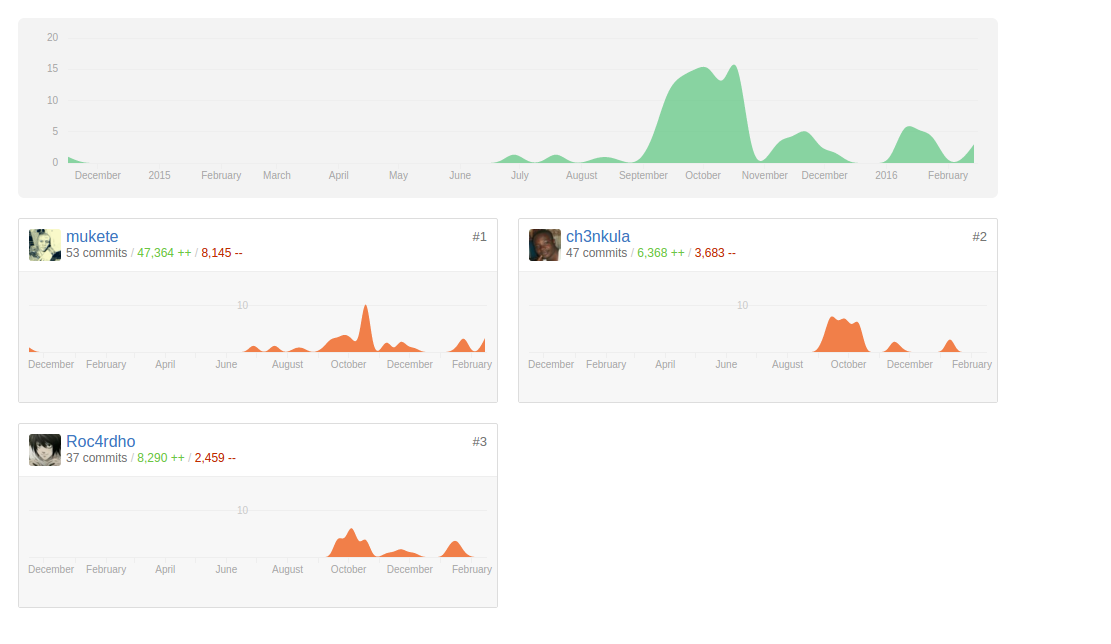
\includegraphics[width=13cm,scale=1.5]{Figures/GitHubProject}
\decoRule
\caption[Nukeboard Code Contributors]{Contributors of codes to Nukeboard}
\label{fig:GitHubProject}
\end{figure}

\subsubsection{General discussion about entire work done}

   Generally, the work I did for 5 months during my internship was a great contribution to the success of this project. Together with my other colleagues, we made sure that when doing a task, we should work on the task very well such that the software in general will be almost perfect and if there is any change we are not make, it will not cost us rebuilding the whole software from scratch. \\
   
In addition to this, we as the nukeboard team worked very much in collaboration both online and offline to make sure that the project goes well and task are accomplished on time and accurately. Also we code in such a way that if a task is given to us and another colleague has to complete it when we are not available, he/she is not stressed up in order to understand the code since its well commented and documented for ease of understanding.

\subsection{Results Obtained}

At this point, results obtained after carrying out all my tasks during my internship period will be revealed. In addition to the above mentioned outcomes(results) where snap-shots where inserted and textual results mentioned, I will also reveal more results here concerning the outcomes as regards my work done during internship.

\subsubsection{Quality Assurance for Nukeboard}

\begin{tabular}{ |p{3cm}|p{3cm}|p{3cm}|  }
 \hline
 \multicolumn{3}{|c|}{Quality Assurance Statistics} \\
 \hline
 Test Cases & \% passed & \% failed \\
 \hline
 53  & 75.47\% & 24.53\% \\
 \hline
\end{tabular}

Testing of the whole software took me 1 month and at the end of the month, I did not still finish testing the whole software but the statistics in the table above reveals the performance and out come of the system including my work and the work of other interns concerning the project.  
%% Chapter 5

\chapter{Conclusion and Recommendations} % Main chapter title

\label{Chapter5} % For referencing the chapter elsewhere, use \ref{Chapter5} 

%----------------------------------------------------------------------------------------

\section{Evaluation of Internship Experience}

\subsection{Self Evaluation}

Evaluating myself, I found out that in even though I had all the skills to work on any programming project, school is complete different from industrial working environment or real life implementation of systems. I realized that its not only about coding or writing little scripts that will perform basic task in your computer. Its about engaging into many things and solving real life problem to provide solutions to the society. Engineering especially software is all about designing, analysis, implementation, maintaining of softwares to help the community grow by solving their problem to easy day to day transaction using softwares and computer programs. \\

In addition to the skills I had before starting internship, I learnt many other technologies and tricks in engineering to problem solving. Communication and working as a team which is a key aspect in engineering was also a great skill that i learnt making me able to work with others from different background of discipline like; Translators, Business Analysts, etc\ldots

In a nut shell, I will conclude by saying that the internship period was a great success and I learnt many things if I had remained in school I wouldn't have known them and also discovered many of my short comings and will make sure that I fix them so I can be better prepared myself for the job environment.

\subsection{Company Evaluation}

This part of the evaluation was done by the owner of the companay in which he filled an evaluation form provided to us by the Faculty in which we have submitted to the faculty. Over all, my evaluation from the company was a good one.

\section{General Conclusion}

To conclude, its a great idea for the facult to give engineering students internship for them to go out to the world and see how the job environment really works. From my experience, I will encourage the faculty to strictly evaluate students on internship because its an opportunity for engineering students to fix all their problems and prepare themselves for the job market. My internship was a success and I really thank everyone that contributed me in one way or the other to develop modules for Nukeboard because it was really indeed a successful one.

\section{Recommendations}

I recommend that the faculty should not change the rule of thumb that students should not do internship because will cause more harm that good since leaving school to the job market without any internship is a real disaster and can jeopardize the reputation of the company if care is not take. So I strongly recommend that internship periods should be taken really seriously because this is the only one opportunity that students have to have a directly relationship with real life companies while still a student.

\section{Furture Works on the project}

There is more work to be done on nukeboard as time goes by and most of these work will be building modules for the software and improving on the nukeboard.co core itself to support new features that will be built on it. Below is a list of up coming features that will be built into the software in the nearest future;\\

- Republishing Jobs Module. \\

- Application text dump that will is stored in the MySQL database will be well formatted and transfered to a different server were search will be done and return as JSON objects since as time goes by, the amount of CV coming in is exponentially big that MySQL database won't be able to handle.\\

- Searching CVs in nukeboard.co will be slow if the amount of CVs grow too large so a different algorithm will be used to speed up the search. A proposed algorithm already was Binary search. \\

- Nukeboard codebase will be refactored and cleaned in order to re-organize the codes and make it really easy to understand so that other developers won't face difficulty in understanding the codes. \\

- etc\ldots

\section{Other projects and work done during internship}

In addition to my work done during internship, I am really amazed at the other tasks I carried out and other technologies I learnt. A quick mention of other things I did during internship is as follows;

- Contributed Codes to Open Source Organisation in PHP(Fixed 25 bugs as of today, 15th Feb 2016). \\

- Worked on other real life projects like; http://efarm.cm(Online Agricultural Market for selling and buying of agricultural products), http://derick-tech.xyz(My Personal Website). \\

- Mentored a Google program(GCI: Google Code In) where students from 13 - 17 years old contribute to open source projects. I mentored under the WMF(Wiki Media Foundation). \\

- Did Freelancing jobs online on Upwork Global Inc and accomplished 10 jobs. \\

- Learnt how to write professional documents in LaTex which uses TeX as the scripting language. I used this technology to write my internship report.\\
 

%----------------------------------------------------------------------------------------
%	THESIS CONTENT - APPENDICES
%----------------------------------------------------------------------------------------

\appendix % Cue to tell LaTeX that the following "chapters" are Appendices

% Include the appendices of the thesis as separate files from the Appendices folder
% Uncomment the lines as you write the Appendices

% Appendix A

\chapter{Appendix Title Here} % Main appendix title

\label{AppendixA} % For referencing this appendix elsewhere, use \ref{AppendixA}

Write your Appendix content here.
%\include{Appendices/AppendixB}
%\include{Appendices/AppendixC}

%----------------------------------------------------------------------------------------
%	BIBLIOGRAPHY
%----------------------------------------------------------------------------------------

\printbibliography[heading=bibintoc]

%----------------------------------------------------------------------------------------

\end{document}  
